\section{Frontend}\label{sec:frontend}

The frontend's purpose is to present the data
it got from the backend to a user
in a manner that is both easy to read
and visually attractive.
Modern frontend applications
are expected to include
fast loading times,
asynchronous data fetching,
intuitive interface,
and some degree of familiarity,
which means they have to resemble
popular services to some extent.

When designing the \ac{UI} for Notipie,
I wanted not only to deliver great visual design,
but also intuitive user experience,
reliability,
and snappiness.
The frontend code
is in the
\texttt{ui} directory~\cite{sewera_notipie_2022-5}.
The \ac{UI} is available both in dark and light mode,
as illustrated in figures~\ref{fig:notipie-ui-dark}
and~\ref{fig:notipie-ui-light} respectively.

\begin{figure}[h]
  \centering
  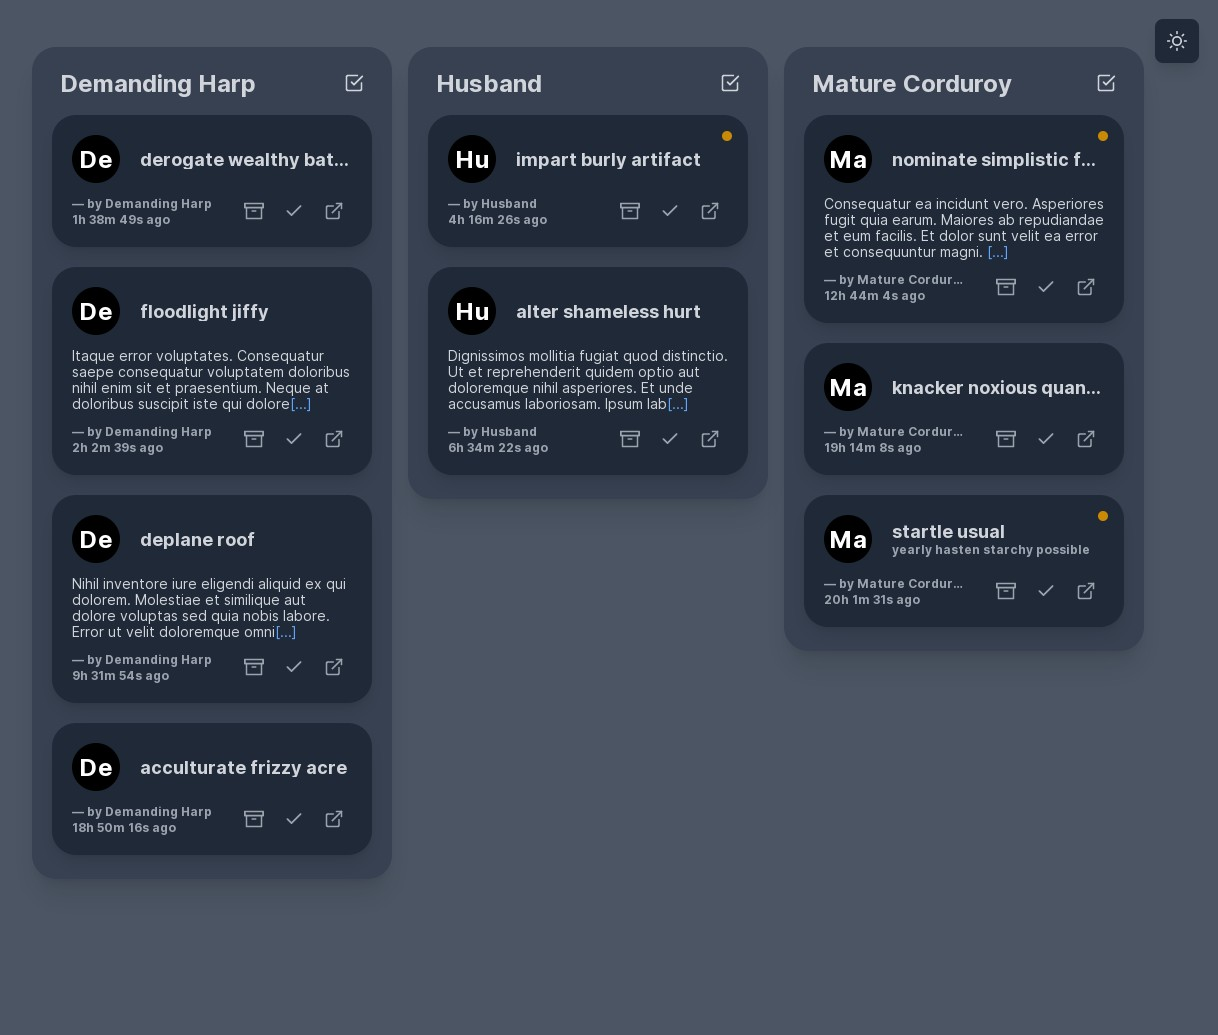
\includegraphics[width=9cm,keepaspectratio]{img/notipie_dark.jpg}
  \caption{Notipie UI: Dark mode}
  \label{fig:notipie-ui-dark}
\end{figure}

\begin{figure}[h]
  \centering
  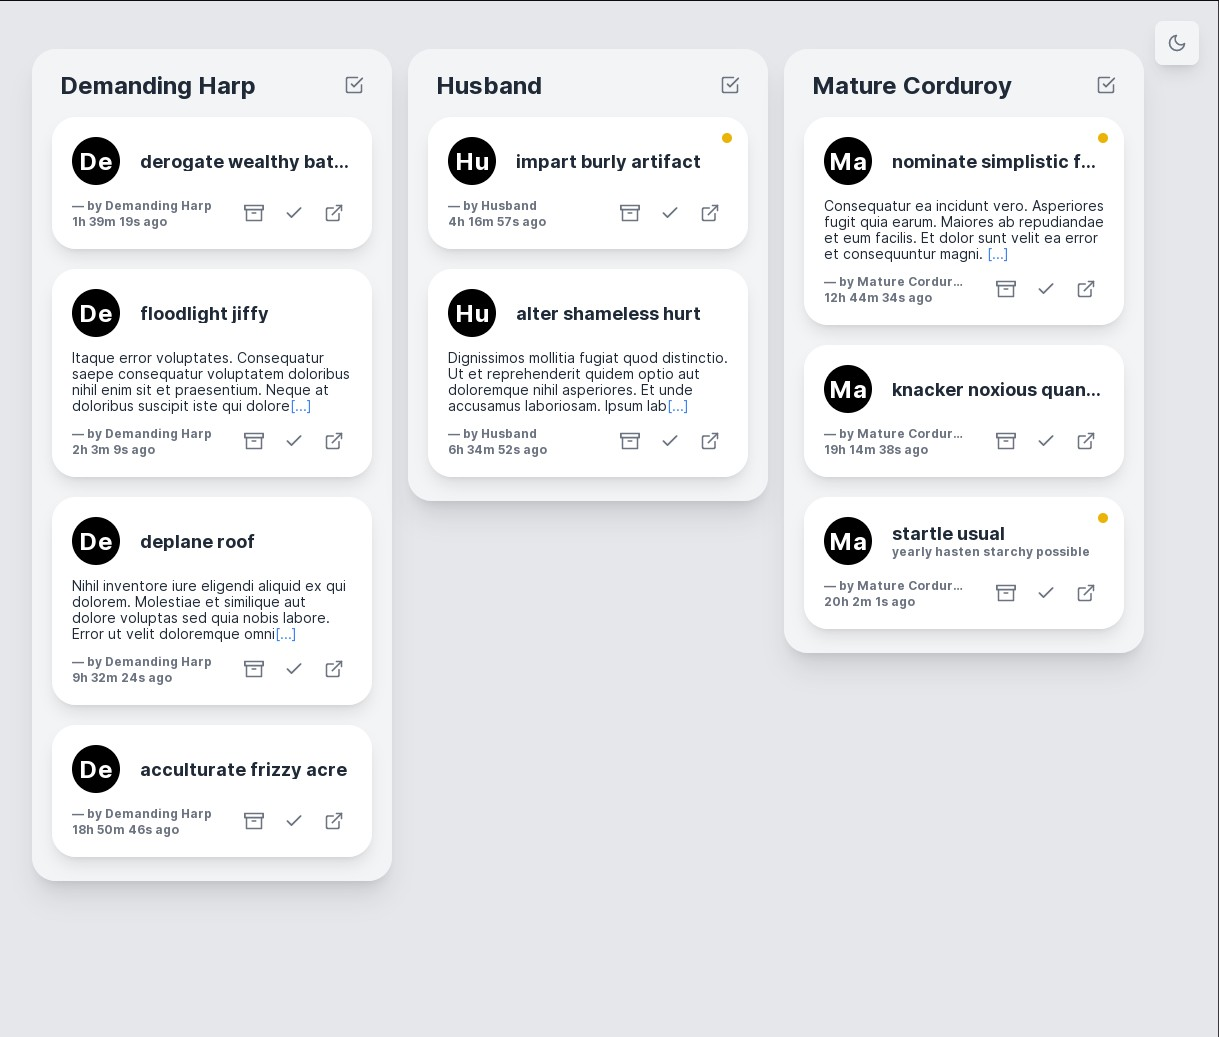
\includegraphics[width=9cm,keepaspectratio]{img/notipie_light.jpg}
  \caption{Notipie UI: Light mode}
  \label{fig:notipie-ui-light}
\end{figure}

\subsubsection{UI Design}\label{sec:ui-design}

When designing the \ac{UI} of Notipie,
I tried to maximize usability
and minimize complexity of the interface.
Maintaining simplicity of the interface is not an easy task,
so I took inspiration from the professional designs.

\paragraph*{Inspirations}\label{sec:inspirations}

My main inspirations for the interface included
Apple Human Interface Guidelines~\cite{apple_inc_human_2022}
and Google's Material Design~\cite{google_llc_material_2022},
but by far the most inspiration was taken from
Github Primer~\cite{github_inc_primer_2022}.
I tried to break down what is useful,
what is unnecessary in my project,
and extract only the essentials for my design.
I began designing with freehand sketching
on my e-book (figure~\ref{fig:early-ui-sketches}).
It allowed me to quickly visualize my ideas
and decide on the elements that I like.

\begin{figure}[h]
      \centering
      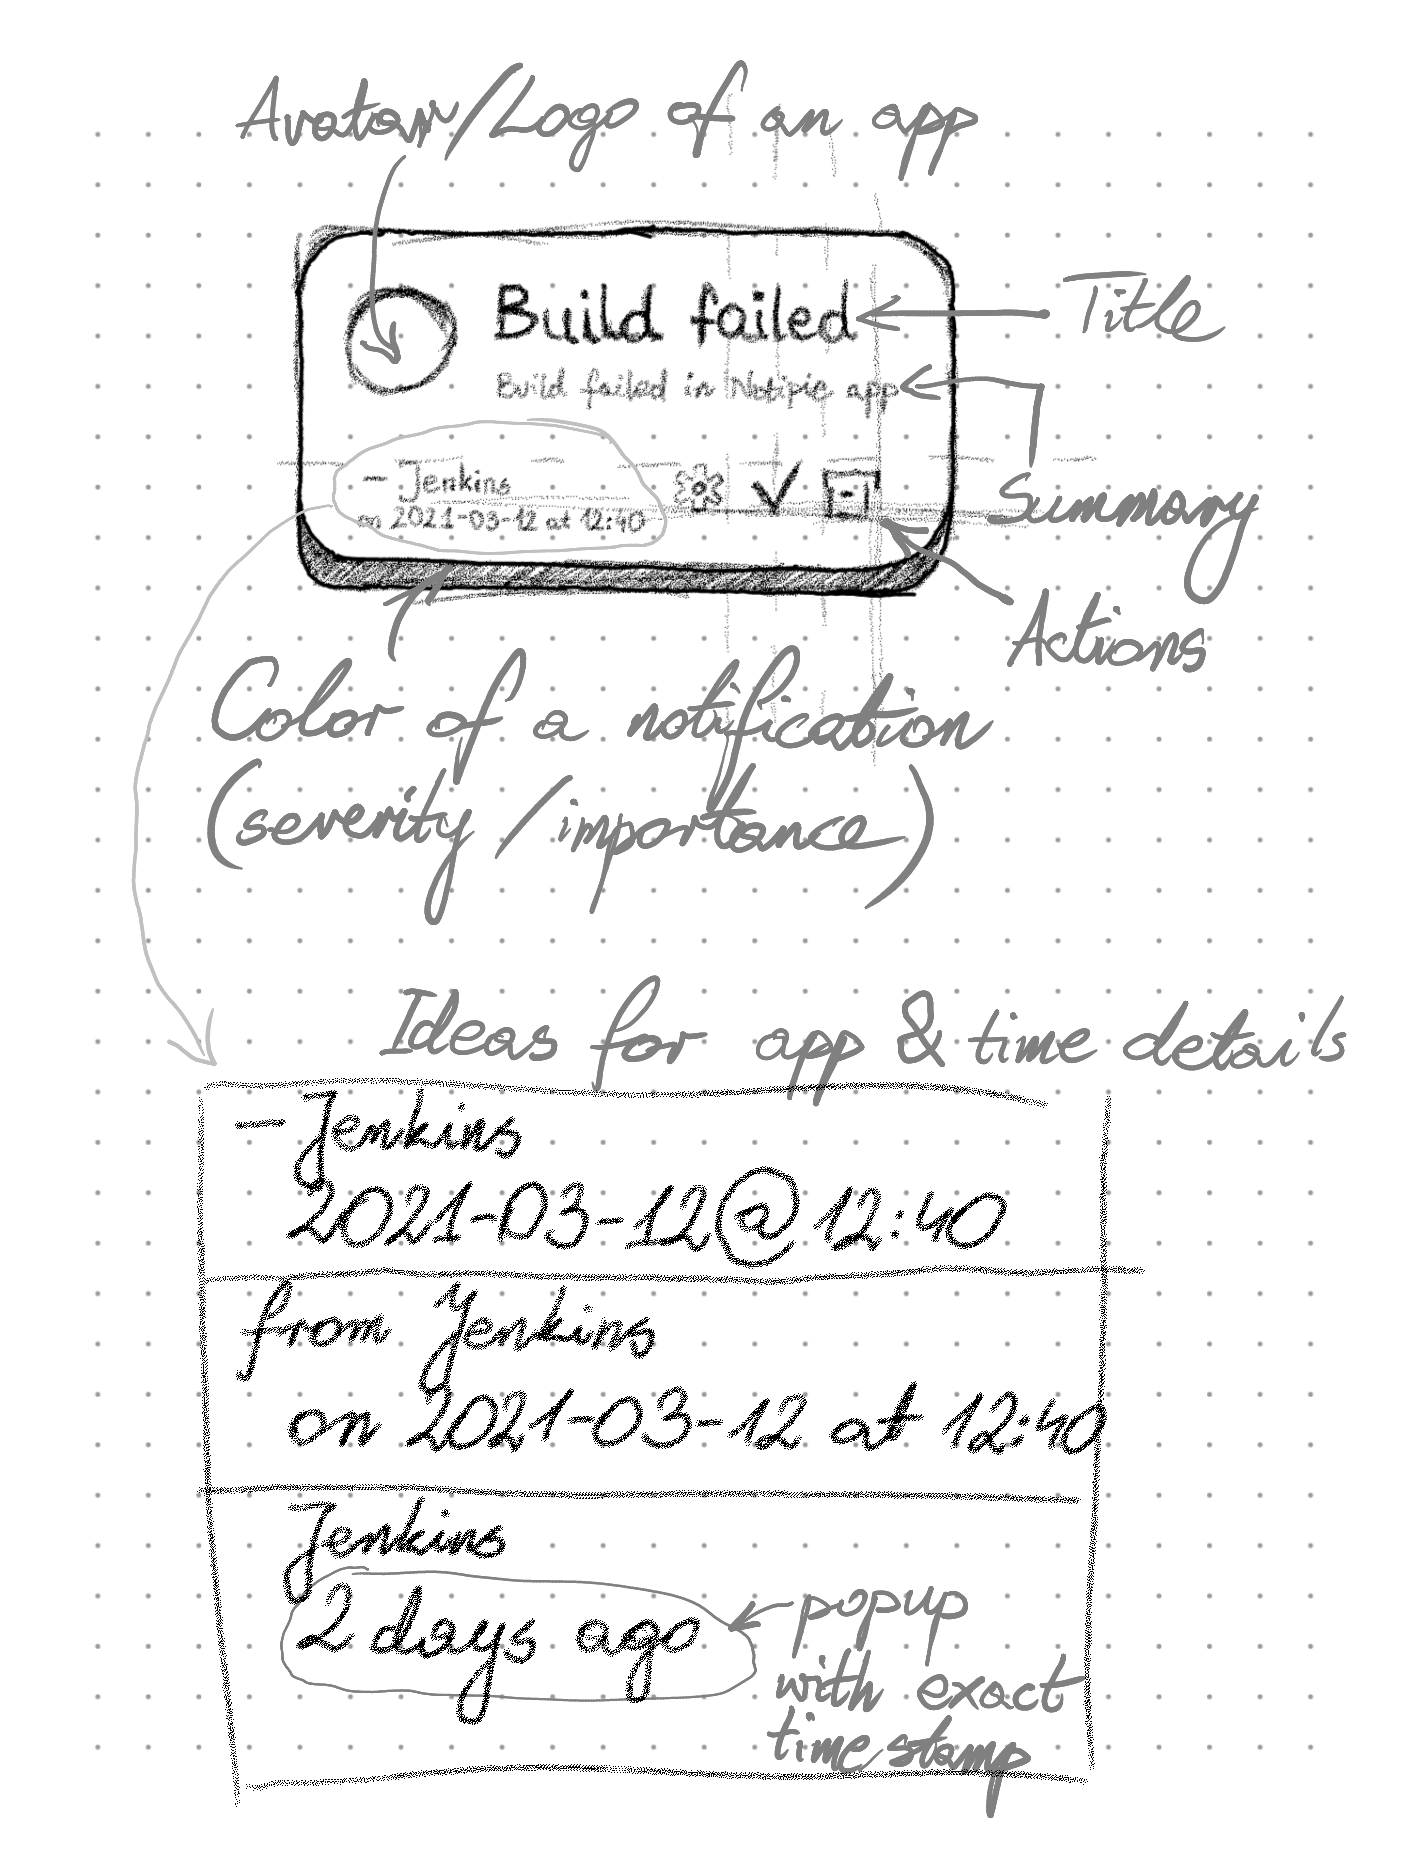
\includegraphics[width=10cm,keepaspectratio]{img/early_ui_sketches.png}
      \caption{Example early sketch made on e-book}
      \label{fig:early-ui-sketches}
\end{figure}

The works of Adam Wathan and Steve Schoger
also had a great influence
on my design decisions.
Their book,
\citetitle{wathan_refactoring_2018}~\cite{wathan_refactoring_2018}
was an excellent guidance on best practices
of modern \ac{UI} design.

\paragraph*{Final design}\label{sec:final-design}

The card is a building block for the entire \ac{UI}.
It provides the most interaction in the whole application,
therefore it had to be designed with a clear information layout
and intuitive controls.
The card itself consists of several elements,
as depicted in figure~\ref{fig:card-with-labeled-elements}:

\begin{enumerate}
      \item
            logo,
            it can be an image
            or automatically generated \ac{SVG}
            from the first two letters of the app's name,
      \item
            indicator,
            whether the notification has been seen or not,
      \item
            title of the notification,
      \item
            subtitle,
      \item
            body,
            which collapses after it reaches a certain length,
            so that an ellipsis appears (\texttt{...}),
      \item
            information about what app sent the notification and when it happened,
      \item
            controls to archive,
            mark as read,
            or go to external site connected with the notification,
            like a certain build on Jenkins,
            or the notification page on Github.
\end{enumerate}

The card was also designed with aesthetics in mind.
All elements were carefully positioned and aligned,
so they are not only pleasant to look at,
but also have features important for visual communication.
Those features, highlighted in figure~\ref{fig:card-with-guides}, include:

\begin{itemize}
      \item
            the rounded corners take the focus away from the card frame,
            and provide a natural, neutral enclosure for the notification,
      \item
            the inner padding is of equal size in each direction
            to provide optical stability,
      \item
            the distance between the logo and title -- subtitle combo
            is the same size as the padding,
            making the logo appear centered,
      \item
            the title -- subtitle combo itself
            is centered vertically relative to the logo,
      \item
            the distances between the logo,
            notification body, and app name -- timestamp combo are shorter
            in order to make the inner section more connected,
      \item
            the controls are centered relative to the app name -- timestamp combo,
      \item
            the \textit{unread} indicator is unobtrusive enough
            not to steal all the focus from the card's content,
      \item
            finally, the \textit{unread} indicator
            is positioned slightly outside the inner section,
            so that it belongs to the card itself,
            not its content,
            therefore it is easier to spot at a glance.
\end{itemize}

\begin{figure}[p]
      \centering
      \begin{minipage}{0.45\textwidth}
            \centering
            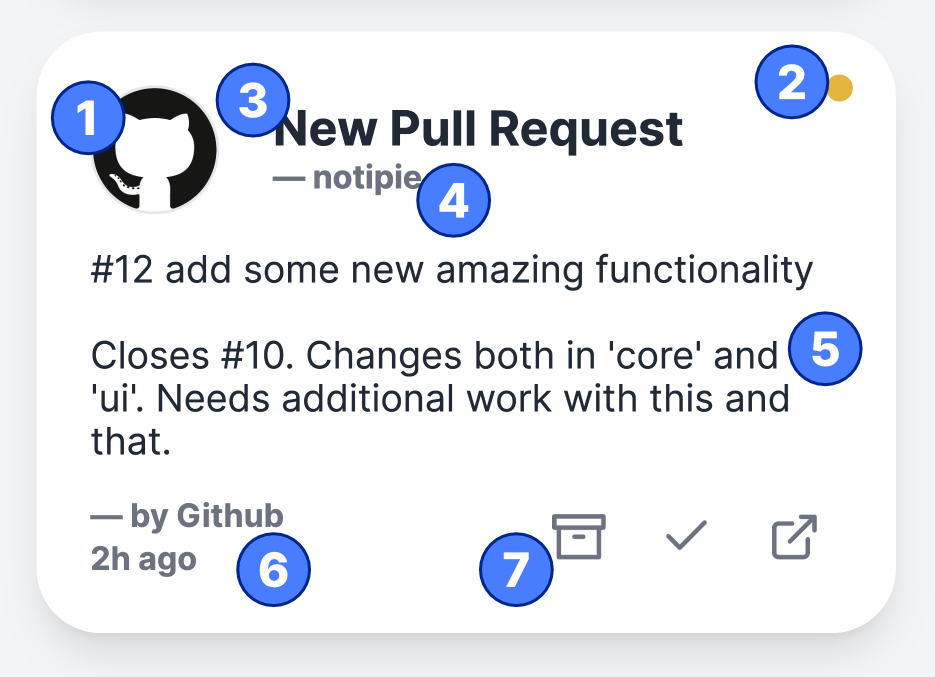
\includegraphics[width=0.9\textwidth,keepaspectratio]{img/card_labeled.png}
            \caption{Card with labeled elements}
            \label{fig:card-with-labeled-elements}
      \end{minipage}\hfill
      \begin{minipage}{0.45\textwidth}
            \centering
            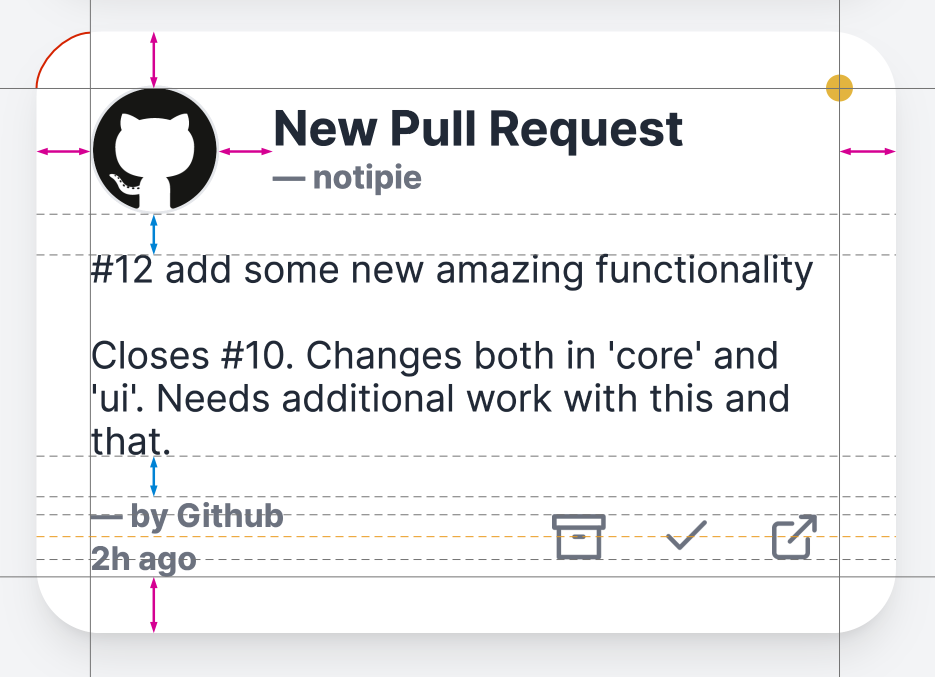
\includegraphics[width=0.9\textwidth,keepaspectratio]{img/card_guides.png}
            \caption{Card with guides}
            \label{fig:card-with-guides}
      \end{minipage}
\end{figure}

\subsubsection{UI components}\label{sec:ui-components}

Using components enabled me to split my \ac{UI}
into small, reusable components,
eliminating code duplication,
and helping maintain consistent look.
I wanted to choose the right library
for this task,
so that the development would be quick,
and I would have plenty of tools
that would help me achieve
good architecture for the frontend.

\paragraph*{UI component library}\label{sec:ui-component-library}

A \ac{UI} component library is a \acf{JS} or \acf{TS} library
enabling a programmer to reduce duplication
in the frontend codebase.
It provides a way to split the frontend code into components,
which can be parametrized, reused, and composed into an entire application,
and to declaratively describe
the appearance and behavior of those components
with a~help of functions or classes.
When choosing the library for the \ac{UI} components, I~considered:

\begin{itemize}
  \item
        React~\cite{oshannessy_react_2022},
  \item
        Vue.js~\cite{you_vuejs_2022}, and
  \item
        Angular~\cite{kalpakas_angular_2022}.
\end{itemize}

All those libraries are very popular,
so I chose React,
because I had the most experience with it in my professional work.

\paragraph*{The component directory}\label{sec:the-component-directory}

All of the frontend components
are located in the component directory~\cite{sewera_notipie_2022-3}.
The directories are divided by category.
There are currently two categories,
\textit{canvas}, and
\textit{notification}.
Canvas category includes
an \texttt{AppCanvas} component,
which is responsible for displaying
a background in the right color,
and controlling the light or dark mode setting.
Notification category includes
a notification card,
a notification container,
which contains all the notifications
from the same App\footnote{
  The concept of an App is described
  in section~\ref{sec:app}.
}, and a notification board,
containing all the notifications
presented in the \ac{UI}.

\paragraph*{Styling}\label{sec:ui-styling}

In addition to the correct behavior of the \ac{UI},
I needed to bring my design of the card\footnote{
  The design of the card
  is explained in detail
  in section~\ref{sec:final-design}.
} and other components
into reality.
I had some experience with Bootstrap~4~\cite{otto_bootstrap_2018},
but I did not like the look of it,
and on top of that,
customizability was complicated.
I also had experience with plain \ac{CSS},
but I did not want additional hassle
of maintaining both \ac{JS} and \ac{CSS}.

I decided I will use a \ac{CSS} utility library,
which will remove additional effort
of manual \ac{CSS} management,
as well as provide me with the necessary tools
to implement my own, custom design.
Tailwind~CSS~\cite{wathan_tailwind_2022}
was my first and only choice.
Not only is it very popular,
but also the documentation is excellent,
there are many tutorials on YouTube,
and it was written by the authors
of \citetitle{wathan_refactoring_2018}~\cite{wathan_refactoring_2018},
one of the books that influenced
my style of design overall,
mentioned also in section~\ref{sec:inspirations}.

\paragraph*{Testing}\label{sec:ui-testing}

\Ac{UI} visual testing tends to be very expensive,
both in terms of time and money.
I used Applitools Eyes~\cite{applitools_applitools_2022}
in my professional work,
and it was both slow,
and the tests were flaky.
I also did not want to spend any money
on the application development.

I used Jest~\cite{bekkhus_jest_2022} for unit tests,
and I was very content with it.
I found out that it has
a \textit{snapshot testing} capability~\cite{bekkhus_snapshot_2022}.
In addition to a \ac{CSS} utility library
like Tailwind~CSS,
I could be fairly sure
that if all \ac{HTML} classes stayed the same,
the look of the entire application
will stay the same.

The snapshot tests were very quick
and easy to review.
The were also easy to debug,
whenever there was some unwanted change.
Coupled with Tailwind~CSS,
they provided a very powerful tool
for regression testing.

\paragraph*{Storybook}\label{sec:storybook}

Another tool that helped with
component creation in isolation
was Storybook~\cite{shilman_storybook_2022}.
The isolation of components
helped with testing,
improved portability and reusability,
and helped me gather all the properties
of each component into an interactive
documentation.
It provided a convenient component library browser,
which worked both in dark and light mode.
The Storybook for Notipie is presented
for dark and light modes in
figures~\ref{fig:storybook-dark}
and~\ref{fig:storybook-light}
respectively.

\begin{figure}[hp]
  \centering
  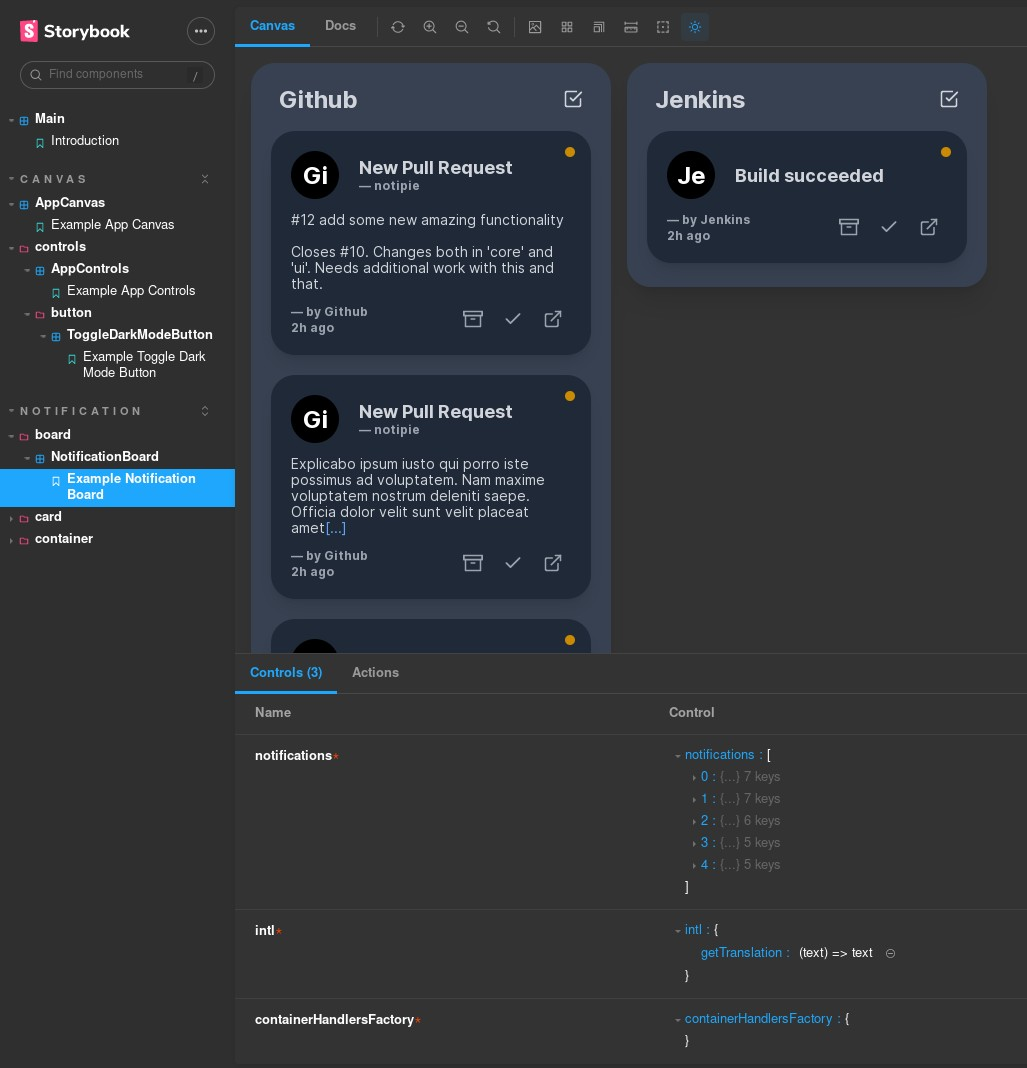
\includegraphics[width=\linewidth,keepaspectratio]{img/storybook.jpg}
  \caption{Storybook for Notipie: Dark mode view}
  \label{fig:storybook-dark}
\end{figure}

\begin{figure}[hp]
  \centering
  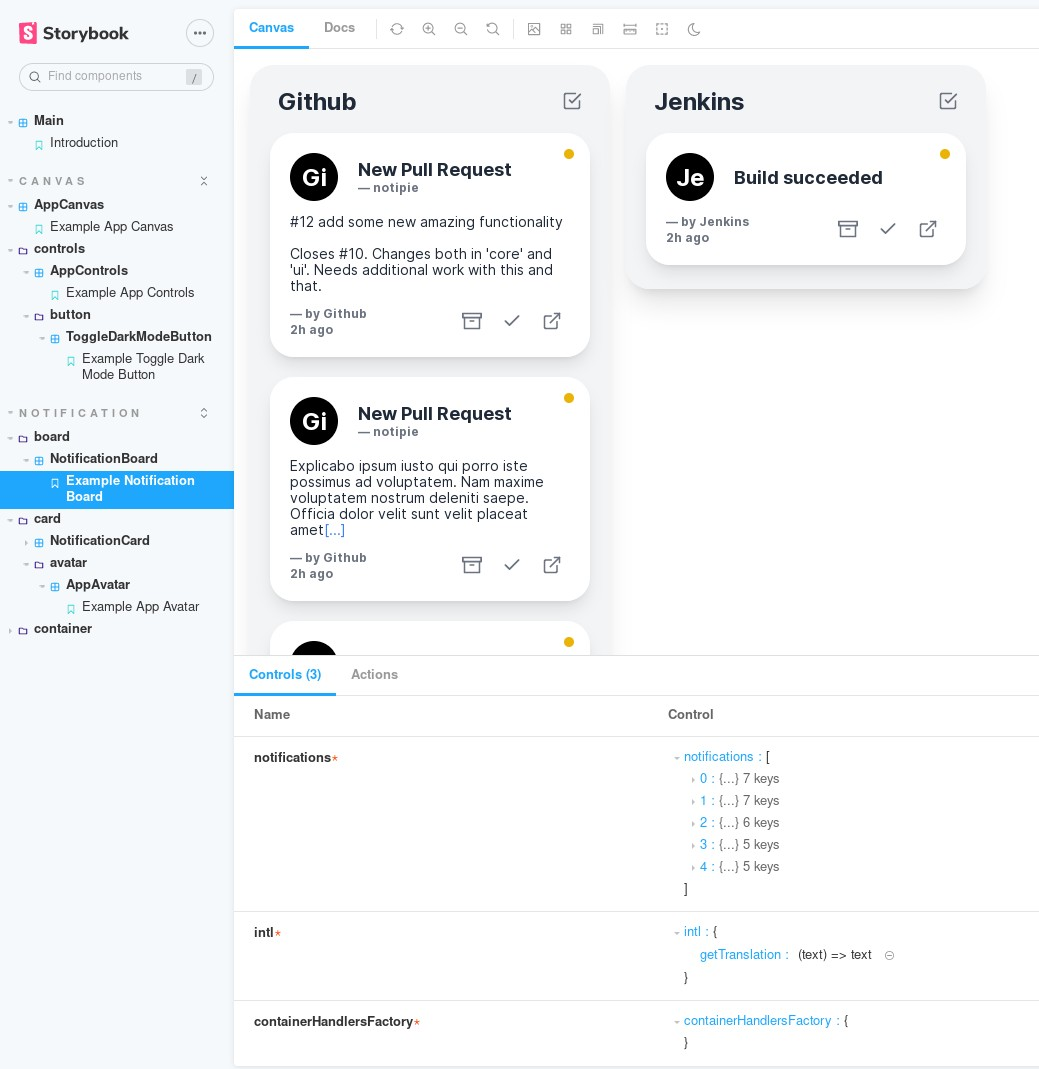
\includegraphics[width=\linewidth,keepaspectratio]{img/storybook_light.jpg}
  \caption{Storybook for Notipie: Light mode view}
  \label{fig:storybook-light}
\end{figure}

\subsubsection{UI networking}\label{sec:ui-networking}

The nature of notifications required me to use
both \ac{REST} data fetching and asynchronous data pushes from the backend.
For the latter, I decided to use \ac{WS},
a standard defined in RFC6455~\cite{fette_rfc6455_2011}, and
RxJS~\cite{lesh_rxjs_2022}, an implementation of
ReactiveX library~\cite{gross_reactivex_2021}.

\paragraph*{REST data fetching}\label{sec:rest-data-fetching}

I used simple \ac{REST}~\cite{perrier_rest_2022} requests
for fetching the notifications
that are already on the backend server.
The standard Fetch browser \ac{API}~\cite{perrier_fetch_2022}
was sufficient for the task.

\paragraph*{Reactive Raven}\label{sec:reactive-raven}

This project~\cite{sewera_reactive_2022} was an experiment
on using RxJS for all real-time data fetching,
enabling the separation of concerns in the code,
and decoupling the state management implementation
from the networking implementation.
When searching for the optimal solution
for pushing the data to the \ac{UI},
I came across two major solutions:

\begin{itemize}
      \item
            Redux Thunk~\cite{gaeraon_redux_2022-1} --
            enough for fetching data on user interaction,
            e.g., on a button click,
            but it provides virtually full implementation lock-in
            to the Redux store, and very little separation of concerns.
            Fetching data is an action dispatched on a store,
            so external communication and storing data are dependent on each other.
      \item
            Redux Saga~\cite{elouafi_redux_2022} --
            good for managing side effects with plain \ac{JS},
            but it uses generator functions
            that yield a different type every time,
            so it is very problematic to use with strict \ac{TS}.
\end{itemize}

Unfortunately,
Thunks and Sagas did not provide the separation of concerns
I wanted to achieve.
Fetching or acting upon pushed data
is a different concern than storing it.
Both had a strict dependency on Redux
store implementation,
so I discarded them as an unacceptable risk
of relying on libraries I could not change.

As a user,
I should not have to dispatch an action on a store
when I want to fetch data.
Of course, the data can be immediately stored after fetching,
but this behavior should be injected later,
so that there is no store implementation lock-in.
The separation of concerns created by using RxJS
enabled me to migrate from Redux to Zustand
as my store implementation,
as described in the next section.

\subsubsection{State management in UI}\label{sec:state-management-in-ui}

To simplify the frontend code,
I needed to use a single source of truth for the data.
Store,
which is a solution for state management
in frontend applications,
is~a~Singleton~\cite{gamma_design_1994}
that can be read by any component,
but can be mutated only using certain functions,
or, in Redux library's case, dispatching actions.
This~approach prevents any data races
or having the store in an unstable state.
I~used both Redux~\cite{gaeraon_redux_2022},
and Zustand~\cite{kato_zustand_2022} for this task
as store implementations,
and Zustand came on top as a simpler solution for my application.

\paragraph*{Redux}\label{sec:redux}

Redux is great for big applications with lots of components.
Being one of the most popular state management libraries for React,
it was my first choice.
Unfortunately,
it required me to write a lot of boilerplate code,
and thus was not easily maintainable
for a smaller project like Notipie.

\paragraph*{Zustand}\label{sec:zustand}

Zustand is a lot simpler than Redux,
requires a lot less boilerplate code,
and was sufficient for my application.
I migrated to it in commit
\texttt{7677d13}\footfullcite{sewera_choreui_2022},
and it reduced the lines of code by over 200.
I did not, however, give up the connected components,
as they provide better testability and separation of concerns,
which is worth a bit extra code.

\addtocategory{commit}{sewera_choreui_2022}

\subsubsection{TypeScript in UI}\label{sec:typescript-in-ui}

There are many tools that can help with maintaining
a frontend codebase.
Linters,
static checkers,
or libraries enforcing certain type at runtime,
just to name a few.
For many years,
we had no other choice but to use
\ac{JS} in frontend projects.
\Acl{TS} is by far the most valuable tool that helps
with making the code maintainability easier.
I decided to use it in my project for the frontend part,
because of its type checking tools,
huge popularity,
and a growing demand for it on the job market.

\paragraph*{Choosing the language}\label{sec:choosing-the-language}

When choosing which language to use in the \ac{UI},
I considered a couple of options:

\begin{itemize}
  \item
        plain \acl{JS},
  \item
        \acl{TS},
  \item
        Elm, and
  \item
        CoffeeScript.
\end{itemize}

I immediately discarded the last two
due to their smaller popularity,
compared to \acl{JS} or \acl{TS}.
Elm and CoffeeScript may have seen
a spike of popularity before \acl{TS}
became main stream,
but as of today,
they have a minuscule market share.

The feature set of the language was also very important to me.
\Acl{JS} is by far the most popular,
but it lacks type annotations or pre-runtime type checking.
\Acl{TS} and Elm turned out to be winners in the type checking toolchain.
\Acl{TS} also has a big advantage of being very similar to plain \acl{JS},
so the transpiled code is very readable.

A big factor was general trend of language's popularity growth.
\Acl{TS} was a clear winner in this scenario,
being third most loved language
and second most wanted language
in the Stack Overflow Developer Survey 2021~\cite{stack_overflow_2021_2021}.
It was only beaten by Rust and Clojure
in the \textit{Most Loved} section,
both of which are non-frontend languages,
and Python in the \textit{Most Wanted} section,
which is also not a frontend language.
Another report confirming the growing popularity of \acl{TS}
is Github Octoverse Report 2021~\cite{github_inc_2021_2021}.
Since 2017,
it beat
Ruby,
C,
C++,
C\#,
Shell, and
\ac{PHP}
and is, as of 2021, the fourth top language on Github.

\paragraph*{Working with TypeScript}\label{sec:working-with-typescript}

Starting with \acl{TS} was fairly easy.
The toolchain was included in the project creation scripts.
Most dependencies had good \acl{TS} annotations,
or they were completely written in \acl{TS},
which was very helpful for maintaining type safety.

Learning the language was also very easy.
I was already familiar with \acl{JS},
so I only needed to learn
the syntax of type annotations,
which were very intuitive to use.
I also found out that because of the type annotations,
function composition became much easier,
so I had less problem working with more complex
language structures.
\Acl{TS} made writing code easier than \acl{JS}.

\subsubsection{Build system}\label{sec:build-system}

For the build and bundle software,
I wanted to use something modern,
with hot module reloading,
easy to use setup scripts,
customizable development server,
and short bundle times.
One library I immediately ruled out
because of lack of those modern features
was Webpack~\cite{koppers_webpack_2022}.
It is a tool with a lot of legacy,
which brought \ac{JS} bundling to the main stream.
However, today its legacy gets in the way
of a clean \ac{API} and good developer experience,
compared to more modern tools.

\paragraph*{Snowpack and Vite}\label{sec:snowpack-and-vite}

I started with Snowpack~\cite{schott_snowpack_2021}
and used it until I decided to move to Vite~\cite{you_vite_2022}
in commit \texttt{c11bc35}\footfullcite{sewera_choreui_2021}.
Snowpack offered both hot module reloading and short bundle times.
Nevertheless,
there were some minor glitches and bugs from time to time,
the project had a slow development,
small user base,
and the alternative, Vite,
did not seem to have those problems.

I tried Vite in my other project,
Reactive Raven~\cite{sewera_reactive_2022},
and the integration with
React,
\ac{TS},
Tailwind~CSS,
and other tools I used was seamless,
therefore I decided to migrate to it in Notipie as well.
On April 20th, 2022,
Snowpack's maintainer stated in the project's Readme document
(commit \texttt{45456aa}\footfullcite{schott_readmemd_2022})
that he would no longer maintain the project,
and mentioned Vite as a good alternative for it.

\addtocategory{commit}{sewera_choreui_2021,schott_readmemd_2022}

